\newpage
\section{Inverting a card}
\genHeader
\hypertarget{sec:invertCard}{}

If you've ever done a swap method before, you'll know you need a temporary variable, some sort of place holder object to store information, to keep it from
being lost.

This next SDM \emph{inverts} a card by swapping its back and face values (Fig.~\ref{fig:goal_invert}). This therefore ``turns a card around'' in the learning
box. This action makes sense if a user wants to try learning, for example, the definition of a word in the opposite direction. Instead of guessing the
definition of every word when presented with the term, perhaps they would like to guess the term when presented with the defintion. This method doesn't need to
accept any parameters - it'll use a bounded \texttt{this} variable.

\vspace{0.5cm}

\begin{figure}[htbp]
	\centering
    \includegraphics[width=0.4\textwidth]{goal_invert.pdf}
 	\caption{Inverting the attributes of a \texttt{Card}}
 	\label{fig:goal_invert}
\end{figure}
\FloatBarrier

% to set the attributes of a temporary card, \texttt{temp} in order to swap the attributes of \texttt{this}.
Something new that we'll use in this SDM are \emph{assignments}\define{Assignments}to set the attributes of \texttt{temp} in \texttt{Initialize temp} and to
swap the attributes of \texttt{this} in \texttt{Swap variables}. An assignment is an attribute constraint with a `\texttt{:=}' operator. Though it might be
slightly confusing to refer to an assignment as a constraint, if you think about it, \emph{everything} can be viewed as different constraints, fulfilled using
different strategies. 

With \texttt{invert}, an assignment is achieved not by searching for a match (as you would with an assertion (\texttt{==, >, <, \ldots}), but
by \emph{performing} the assignment. Similarly, non-context elements (set to create or destroy) can be viewed as structural constraints that are fulfilled by
creating or destroying the corresponding element.  A constraint is therefore a unifying concept similar to ``everything is an object'' from OO, and ``everything
is a model'' from metamodelling.  If you're interested in why \emph{unification} is considered cool check out \cite{BEZ05}.

% % move to start of the next SDM? ---------------------------------------------------------------------------------------------------------------  
% Before we move on, lets mention one last point.  Did you notice that \texttt{temp} is bound in the \texttt{Swap variables} story pattern?  This is a new case
% for bound variables that we haven't treated yet!

% Until now, we have seen object variables that can be (1) bound to an argument of the method that is set when the method is invoked, or (2) bound to the
% current object \texttt{this} whose method is invoked. In both cases, the object to be matched is completely determined by the context of the method and does
% not need to be determined at random by the pattern matcher.

% Setting \texttt{temp} as bound in \texttt{Swap variables} is a third case in which an object variable is bound to the value already determined in a
% \emph{previous} activity node. This means that in this SDM, the object variable \texttt{temp} in \texttt{Swap variables} is to be bound to the value
% determined for the unbound object variable \texttt{temp} in \texttt{Initialize temp}. This binding always enables you to refer to previous matches for object
% variables in the preceding control flow.

% Please note that the reference, or mapping, is implicitly defined via the same \emph{name} of the object variable. With the arguments of this method, the
% editor provides rudimentary support via a drop-down menu which can be used to choose the name of an object variable and avoid possible mistakes stemming from
% typing by hand.


\fancyfoot[R]{ $\triangleright$ \hyperlink{invertCard vis}{Next [visual]\hspace{0.2cm} } \\ $\triangleright$ \hyperlink{invertCard tex}{Next [textual]} }

\newpage
\subsection{Implementing invert}
\visHeader
\hypertarget{invertCard vis}{}

\begin{itemize}

% Make sure you explain how/why the green box. Hasn't been convered yet
\item[$\blacktriangleright$] Model the SDM depicted in Fig.~\ref{fig:sdm_invert}. Remember, the green creational object variable is made by setting the binding
operator as \texttt{create}.

% Explain how to use the new assignments??

\vspace{1cm}

\begin{figure}[htbp]
\begin{center}
  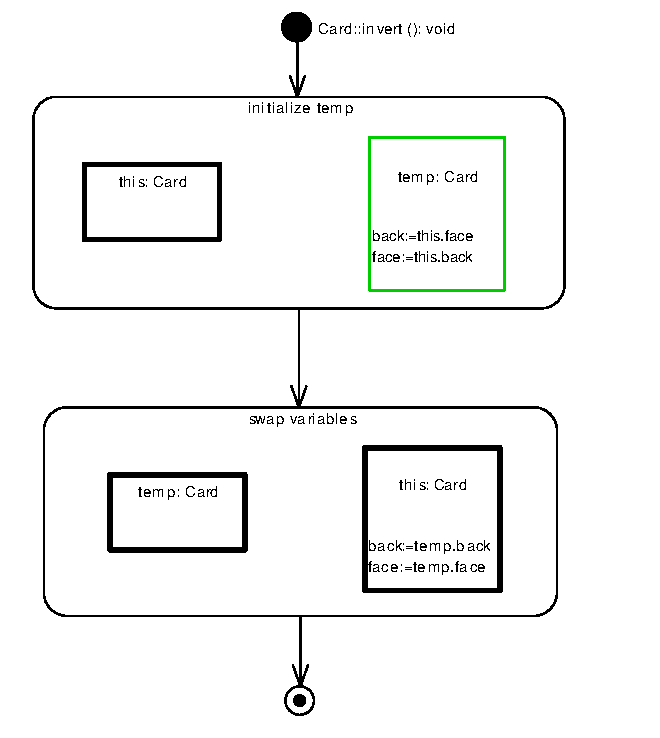
\includegraphics[width=0.9\textwidth]{ea_swappingCard.pdf}
  \caption{Swap back and face of the card}  
  \label{fig:sdm_invert}
\end{center}
\end{figure}

\item[$\blacktriangleright$] Believe or not, that's it! Check out how this method was implemented in the textual syntax by reviewing
Fig.~\ref{fig:invertPatterns} in the next section.

\end{itemize}


\newpage
\subsection{Textual; Turning Cards}
\texHeader
\hypertarget{invertCard tex}{}

\begin{itemize}

\item[$\blacktriangleright$] You're no longer an SDM beginner, so create two patterns in the invert declaration, named \texttt{initializeTemp} and
\texttt{swapVariable}. The only flow this method requires is that these pattern are performed in order - there's no assertion, and it only needs to be
performed once. Don't forget to include a return statement!

\item[$\blacktriangleright$] Your declaration should now resemble Fig.~\ref{fig:eclipse_invert}

\begin{figure}[htbp]
\begin{center}
  \includegraphics[width=0.4\textwidth]{eclipse_invertControlFlow}
  \caption{Control flow for \texttt{card.invert}}  
  \label{fig:eclipse_invert}
\end{center}
\end{figure}

\item[$\blacktriangleright$] Create two bounded object variables in each pattern, and complete the rules until your patterns resemble
Fig.~\ref{fig:invertPatterns}.

\begin{figure}[htbp]
\begin{center}
  \includegraphics[width=0.5\textwidth]{eclipse_invertPatterns}
  \caption{Swap Patterns}  
  \label{fig:invertPatterns}
\end{center}
\end{figure}

\item[$\blacktriangleright$] Believe it or not, that's it! We reccommend building at this point, just to confirm nothing has gone wrong with your metamodel. To
see this method in the visual syntax, review Fig.~\ref{fig:sdm_invert}.

\end{itemize}
